\documentclass[a4paper,10pt]{article}
%-----------------------------------------------------------
\usepackage[top=0.75in, bottom=0.75in, left=0.55in, right=0.85in]{geometry}
\usepackage{graphicx}
\usepackage{url}
\usepackage{palatino}
\usepackage{tabularx}
\usepackage{multirow}
\fontfamily{SansSerif}
\selectfont

\usepackage[T1]{fontenc}
\usepackage
%[ansinew]
[utf8]
{inputenc}

\usepackage{color}
\definecolor{mygrey}{gray}{0.75}
\textheight=9.75in
\raggedbottom

\setlength{\tabcolsep}{0in}
\newcommand{\isep}{-2 pt}
\newcommand{\lsep}{-0.5cm}
\newcommand{\psep}{-0.6cm}
\renewcommand{\labelitemii}{$\circ$}

\pagestyle{empty}
%-----------------------------------------------------------
%Custom commands
\newcommand{\resitem}[1]{\item #1 \vspace{-2pt}}
\newcommand{\resheading}[1]{{\small \colorbox{mygrey}{\begin{minipage}{0.975\textwidth}{\textbf{#1 \vphantom{p\^{E}}}}\end{minipage}}}}
\newcommand{\ressubheading}[3]{
\begin{tabular*}{2in}{l @{\extracolsep{\fill}} r}
	\textsc{{\textbf{#1}}} & \textsc{\textit{[#2]}} \\
\end{tabular*}\vspace{-8pt}}

\title{cv}
\author{manishdalal }
\date{October 2017}

\begin{document}

\begin{tabular*}{6.25in}{l@{\extracolsep{\fill}}r}
  \textbf{\Large Manish Dalal }  \\
    Vill. Kambohpura, P/o: Madhuban\\
    Distt. Karnal, Haryana\\
    Pincode : 132037\\
    Mobile No : \textbf{8395960324} \\
   Email-id : \textbf{manishdalal2016@gmail.com} \\ 
  & \multirow{-8}{*}{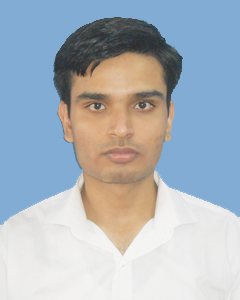
\includegraphics[scale=0.8]{photo.jpg}}\\
  & \\
%-------------------------------------------------
   
\end{tabular*}

\resheading{\textbf{PROFESSIONAL OBJECTIVE} }\\[\lsep]
\begin{itemize}
\item \noindent To work in competitive and challenging environment so as to enhance my knowledge and skills to\\
contribute in the progress of the organization as well as myself.
\end{itemize}

\resheading{\textbf{ACADEMIC DETAILS} }\\[\lsep]
\\ \\
%\begin{table}[ht!]
%\begin{center}
\indent \begin{tabular}{ l @{\hskip 0.45in} l @{\hskip 0.45in} l @{\hskip 0.45in} l @{\hskip 0.35in}  l @{\hskip 0.35in}l }

\hline
\textbf{Qualification} & \textbf{Institute/School} & \textbf{University} & \textbf{Year} & \textbf{Percentage} \\
\hline

B. Tech(pursuing)\,\, & \textit{Seth Jai Parkash Mukand Lal}\,\, & Kurukshetra\,\, & 2018\,\, & 64 \\

& \textit{Institute of Technology, Radaur}\,\, & University \\

Class 12\,\, & \textit{Haryana Police Public}\,\, & CBSE\,\, & 2013\,\, & 66\\
& \textit{School, Karnal}\\

Class 10\,\, & \textit{Haryana Police Public}\,\, & CBSE\,\, & 2011\,\, & 66\\
& \textit{School, Karnal}\\

\hline
\end{tabular}
%\end{center}
%\end{table}
\\ \\

\resheading{\textbf{TECHINICAL SKILLS} }\\[\lsep]
\begin{itemize}
\item \noindent Programming Languages: C, C++, Python and Java
\item \noindent Database: SQL Server 2012 
\item \noindent Operating system: Windows and Linux
\item \noindent Software Packages: MyEclipse, Eclipse and \LaTeX

\end{itemize}

\resheading{\textbf{TRAININGS} }\\[\lsep]
\begin{itemize}
\item \noindent Undergone training in Core java.
\item \noindent Undergone training in Advanced java.
\end{itemize}

\resheading{\textbf{ACADEMIC PROJECTS UNDERTAKEN } }\\[\lsep]
\begin{itemize}
\item \textbf{Online Real Estate Portal: } \\
 \emph{(Guide:Prof. Manoj Dembla.
, June'17 - till date)} \\[-0.6cm]
	\begin{itemize}\itemsep \isep
	\item \textit{Skills Used:} HTML, CSS, JavaScript, JQuery, Servlets, JSP, Java Database Connectivity.
	\item \textit{Description:} The project aims at developing an efficient info management system for real estate \\
	industry. It is online portal for buyer who want to invest in real estate businesses. There would
	\\ 
	be features like user login, registration and browsing properties.

	\end{itemize}

\item \textbf{Chat Express:}\\
 \emph{(Guide: Prof. Manish Bhatia, June'16 - Aug'16)} \\[-0.6cm]
	\begin{itemize}\itemsep \isep
	\item \textit{Skills Used:} Socket Programming, Java swing, Event Handling.
	\item \textit{Description:} Chat Express is chat application provides a real time communication between\\
	two or more users at the same time. It made up of two applications the client application,\\ 
	which runs on the user’s Pc and server application, which runs on any Pc on the network. 
	\end{itemize}
\end{itemize}

\resheading{\textbf{STRENGTHS} }\\[\lsep]
\begin{itemize}
\item \noindent	Continuous learner and willingness to improve with experience.
\item \noindent	Optimum utilize of time with best use of knowledge and technology.
\item \noindent	Curious to explore and learn new things.
\item \noindent Adaptability and Flexibility.
\end{itemize}

\resheading{\textbf{PERSONAL DETAILS} }\\[\lsep]
\begin{itemize}
\item \noindent \textbf{Father’s Name:} Sh. Balvinder Dalal
\item \noindent \textbf{Date of Birth: } 21/10/1995 
\item \noindent \textbf{Marital Status:} Unmarried
\item \noindent \textbf{Hobbies:} Listening music, Solving Puzzles and Playing Cricket \\ \\ \\ 
\end{itemize}
\begin{tabular}{ l @{\hskip 4.5in} l @{\hskip 1in}  }
\indent \textbf{Place: }JMIT, Radaur \,\, & Manish Dalal\\
\indent \textbf{Date}
\end{tabular}
\end{document}

